\phantomsection\label{cec40bd4}
Load Python packages

\phantomsection\label{bd3a6a21}
\nointerlineskip\nointerlineskip\begin{minted}[autogobble,samepage]{python}
import numpy as np
import sympy as sp
import matplotlib.pyplot as plt
import dysys
from pprint import pprint
\end{minted}

\phantomsection\label{4c365de9}

\phantomsection\label{756a411f}
\subsubsection{Define the System}\label{define-the-system}

Define a symbolic state-space matrix using the \mintinline{text}|dysys|
package as follows:

\phantomsection\label{f634d35e}
\nointerlineskip\nointerlineskip\begin{minted}[autogobble,samepage]{python}
A = [[-4, -3, 0], [0, -8, 4], [0, 0, -1]]
B = [[0], [1], [0]]
C = [[0, 1, 0]]
D = [[0]]
sys = dysys.sss(A, B, C, D)  # Create a symbolic state-space model
\end{minted}

\phantomsection\label{c8734e57}
\subsubsection{Eigenvalues and
Stability}\label{eigenvalues-and-stability}

The eigenvalue matrix \mintinline{text}|L| can be found via the eig()
method:

\phantomsection\label{32e3ee2b}
\nointerlineskip\nointerlineskip\begin{minted}[autogobble,samepage]{python}
L, M = sys.eig()
print(f"Eigenvalues: {L.diagonal().tolist()}")
\end{minted}

\nointerlineskip\nointerlineskip\begin{minted}[autogobble,samepage]{text}
Eigenvalues: [[-8, -4, -1]]
\end{minted}

\phantomsection\label{83c9c043}
The real parts of the eigenvalues are all negative; therefore, the
system is asymptotically stable.

\phantomsection\label{867e3e2d}
\subsubsection{Eigenvectors and the Modal
Matrix}\label{eigenvectors-and-the-modal-matrix}

The eigenvectors are stored in \mintinline{text}|M|:

\phantomsection\label{024a5ed7}
\nointerlineskip\nointerlineskip\begin{minted}[autogobble,samepage]{python}
print(M)
\end{minted}

\nointerlineskip\nointerlineskip\begin{minted}[autogobble,samepage]{text}
Matrix([[3/4, 1, -4/7], [1, 0, 4/7], [0, 0, 1]])
\end{minted}

\phantomsection\label{0448c950}
\subsubsection{State Transition Matrix}\label{state-transition-matrix}

The state transition matrix $\Phi(t)$ can be found as follows:

\phantomsection\label{7d9946da}
\nointerlineskip\nointerlineskip\begin{minted}[autogobble,samepage]{python}
t = sp.Symbol("t", nonnegative=True)  ## Solution valid for t >= 0
Phi = sys.state_transition_matrix(t)
pprint(Phi)
\end{minted}

\nointerlineskip\nointerlineskip\begin{minted}[autogobble,samepage]{text}
Matrix([
[exp(-4*t), -3*exp(-4*t)/4 + 3*exp(-8*t)/4, -4*exp(-t)/7 + exp(-4*t) - 3*exp(-8*t)/7],
[        0,                      exp(-8*t),              4*exp(-t)/7 - 4*exp(-8*t)/7],
[        0,                              0,                                  exp(-t)]])
\end{minted}

\phantomsection\label{76bc68e6}
\subsubsection{Forced State Response}\label{forced-state-response}

The forced state response for $t \ge 0$ can be found as follows:

\phantomsection\label{9b10d000}
\nointerlineskip\nointerlineskip\begin{minted}[autogobble,samepage]{python}
u_s = sp.Heaviside(t)
x_fo = sys.state_forced_response(t, u=u_s)
pprint(x_fo)
\end{minted}

\nointerlineskip\nointerlineskip\begin{minted}[autogobble,samepage]{text}
Matrix([
[-3/32 + 3*exp(-4*t)/16 - 3*exp(-8*t)/32],
[                      1/8 - exp(-8*t)/8],
[                                      0]])
\end{minted}

\phantomsection\label{bbd55a21}
\subsubsection{Forced Output Response}\label{forced-output-response}

\phantomsection\label{776c3cb1}
\nointerlineskip\nointerlineskip\begin{minted}[autogobble,samepage]{python}
y_fo = sys.output_forced_response(t, u=u_s)
pprint(y_fo)
\end{minted}

\nointerlineskip\nointerlineskip\begin{minted}[autogobble,samepage]{text}
Matrix([[1/8 - exp(-8*t)/8]])
\end{minted}

\phantomsection\label{91cc4912}
\subsubsection{Plot the Forced Output
Response}\label{plot-the-forced-output-response}

First, convert the symbolic expression to a NumPy function:

\phantomsection\label{f20fc639}
\nointerlineskip\nointerlineskip\begin{minted}[autogobble,samepage]{python}
y_fo_fun = sp.lambdify(t, y_fo, "numpy")
\end{minted}

\phantomsection\label{d99621f3}
Now create arrays to plot:

\phantomsection\label{87da832b}
\nointerlineskip\nointerlineskip\begin{minted}[autogobble,samepage]{python}
t_ = np.linspace(0, 5, 101)
y_fo_ = y_fo_fun(t_).flatten()
\end{minted}

\phantomsection\label{2f6f12db}
Finally, plot:

\phantomsection\label{1aada182}
\nointerlineskip\nointerlineskip\begin{minted}[autogobble,samepage]{python}
fig, ax = plt.subplots()
ax.plot(t_, y_fo_)
ax.set_xlabel("Time (s)")
ax.set_ylabel("Forced Output Response $y_\\text{fo}$")
plt.show()
\end{minted}

\phantomsection\label{0709cb00}
\gdef\graphicslist{}%
\begin{figure}[htbp]
\centering
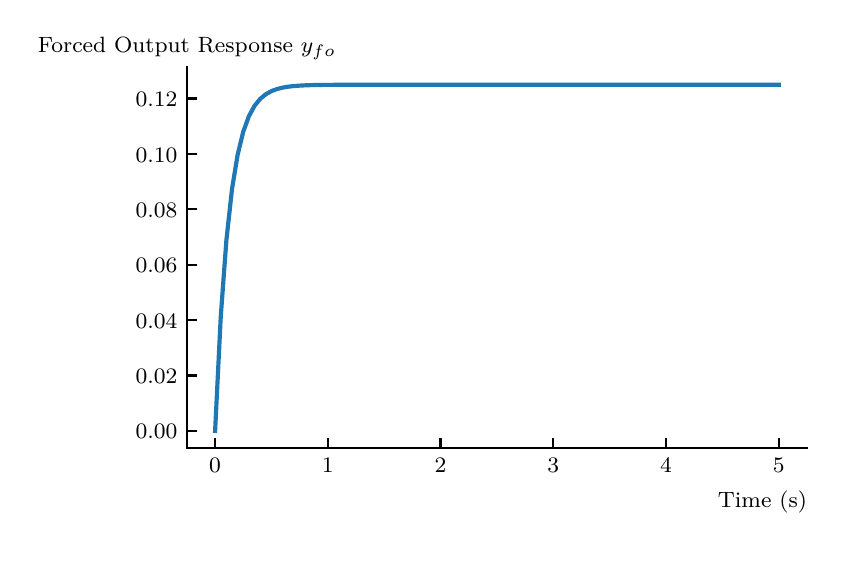
\begin{tikzpicture}%
\node[inner sep=0pt] {%% Creator: Matplotlib, PGF backend
%%
%% To include the figure in your LaTeX document, write
%%   \input{<filename>.pgf}
%%
%% Make sure the required packages are loaded in your preamble
%%   \usepackage{pgf}
%%
%% Also ensure that all the required font packages are loaded; for instance,
%% the lmodern package is sometimes necessary when using math font.
%%   \usepackage{lmodern}
%%
%% Figures using additional raster images can only be included by \input if
%% they are in the same directory as the main LaTeX file. For loading figures
%% from other directories you can use the `import` package
%%   \usepackage{import}
%%
%% and then include the figures with
%%   \import{<path to file>}{<filename>.pgf}
%%
%% Matplotlib used the following preamble
%%   \def\mathdefault#1{#1}
%%   \everymath=\expandafter{\the\everymath\displaystyle}
%%   \RequirePackage[T1]{fontenc}%
%%   \usepackage{newpxmath} % math font is Palatino compatible
%%   \let\Bbbk\relax % so it doesn't clash with amssymb
%%   \usepackage[no-math]{fontspec}
%%   \setmainfont{Palatino}
%%   \setmonofont{Latin Modern Mono}[%
%%   Scale=1.05, % a touch smaller than MatchLowercase
%%   BoldFont=*,
%%   BoldFeatures={FakeBold=2}
%%   ]
%%   \setsansfont{Helvetica}
%%   \renewcommand{\mathdefault}[1][]{}
%%   \usepackage{fontspec}
%%   \setmainfont{Palatino.ttc}[Path=\detokenize{/System/Library/Fonts/}]
%%   \setsansfont{DejaVuSans.ttf}[Path=\detokenize{/Users/ricopicone/anaconda3/envs/dysys/lib/python3.11/site-packages/matplotlib/mpl-data/fonts/ttf/}]
%%   \setmonofont{DejaVuSansMono.ttf}[Path=\detokenize{/Users/ricopicone/anaconda3/envs/dysys/lib/python3.11/site-packages/matplotlib/mpl-data/fonts/ttf/}]
%%   \makeatletter\@ifpackageloaded{underscore}{}{\usepackage[strings]{underscore}}\makeatother
%%
\begingroup%
\makeatletter%
\begin{pgfpicture}%
\pgfpathrectangle{\pgfpointorigin}{\pgfqpoint{3.996259in}{2.529536in}}%
\pgfusepath{use as bounding box, clip}%
\begin{pgfscope}%
\pgfsetbuttcap%
\pgfsetmiterjoin%
\definecolor{currentfill}{rgb}{1.000000,1.000000,1.000000}%
\pgfsetfillcolor{currentfill}%
\pgfsetlinewidth{0.000000pt}%
\definecolor{currentstroke}{rgb}{1.000000,1.000000,1.000000}%
\pgfsetstrokecolor{currentstroke}%
\pgfsetdash{}{0pt}%
\pgfpathmoveto{\pgfqpoint{0.000000in}{0.000000in}}%
\pgfpathlineto{\pgfqpoint{3.996259in}{0.000000in}}%
\pgfpathlineto{\pgfqpoint{3.996259in}{2.529536in}}%
\pgfpathlineto{\pgfqpoint{0.000000in}{2.529536in}}%
\pgfpathlineto{\pgfqpoint{0.000000in}{0.000000in}}%
\pgfpathclose%
\pgfusepath{fill}%
\end{pgfscope}%
\begin{pgfscope}%
\pgfsetbuttcap%
\pgfsetmiterjoin%
\definecolor{currentfill}{rgb}{1.000000,1.000000,1.000000}%
\pgfsetfillcolor{currentfill}%
\pgfsetlinewidth{0.000000pt}%
\definecolor{currentstroke}{rgb}{0.000000,0.000000,0.000000}%
\pgfsetstrokecolor{currentstroke}%
\pgfsetstrokeopacity{0.000000}%
\pgfsetdash{}{0pt}%
\pgfpathmoveto{\pgfqpoint{0.796259in}{0.427040in}}%
\pgfpathlineto{\pgfqpoint{3.896259in}{0.427040in}}%
\pgfpathlineto{\pgfqpoint{3.896259in}{2.330625in}}%
\pgfpathlineto{\pgfqpoint{0.796259in}{2.330625in}}%
\pgfpathlineto{\pgfqpoint{0.796259in}{0.427040in}}%
\pgfpathclose%
\pgfusepath{fill}%
\end{pgfscope}%
\begin{pgfscope}%
\pgfsetbuttcap%
\pgfsetroundjoin%
\definecolor{currentfill}{rgb}{0.000000,0.000000,0.000000}%
\pgfsetfillcolor{currentfill}%
\pgfsetlinewidth{0.803000pt}%
\definecolor{currentstroke}{rgb}{0.000000,0.000000,0.000000}%
\pgfsetstrokecolor{currentstroke}%
\pgfsetdash{}{0pt}%
\pgfsys@defobject{currentmarker}{\pgfqpoint{0.000000in}{0.000000in}}{\pgfqpoint{0.000000in}{0.048611in}}{%
\pgfpathmoveto{\pgfqpoint{0.000000in}{0.000000in}}%
\pgfpathlineto{\pgfqpoint{0.000000in}{0.048611in}}%
\pgfusepath{stroke,fill}%
}%
\begin{pgfscope}%
\pgfsys@transformshift{0.937168in}{0.427040in}%
\pgfsys@useobject{currentmarker}{}%
\end{pgfscope}%
\end{pgfscope}%
\begin{pgfscope}%
\definecolor{textcolor}{rgb}{0.000000,0.000000,0.000000}%
\pgfsetstrokecolor{textcolor}%
\pgfsetfillcolor{textcolor}%
\pgftext[x=0.937168in,y=0.378429in,,top]{\color{textcolor}{\rmfamily\fontsize{8.000000}{9.600000}\selectfont\catcode`\^=\active\def^{\ifmmode\sp\else\^{}\fi}\catcode`\%=\active\def%{\%}$\mathdefault{0}$}}%
\end{pgfscope}%
\begin{pgfscope}%
\pgfsetbuttcap%
\pgfsetroundjoin%
\definecolor{currentfill}{rgb}{0.000000,0.000000,0.000000}%
\pgfsetfillcolor{currentfill}%
\pgfsetlinewidth{0.803000pt}%
\definecolor{currentstroke}{rgb}{0.000000,0.000000,0.000000}%
\pgfsetstrokecolor{currentstroke}%
\pgfsetdash{}{0pt}%
\pgfsys@defobject{currentmarker}{\pgfqpoint{0.000000in}{0.000000in}}{\pgfqpoint{0.000000in}{0.048611in}}{%
\pgfpathmoveto{\pgfqpoint{0.000000in}{0.000000in}}%
\pgfpathlineto{\pgfqpoint{0.000000in}{0.048611in}}%
\pgfusepath{stroke,fill}%
}%
\begin{pgfscope}%
\pgfsys@transformshift{1.500804in}{0.427040in}%
\pgfsys@useobject{currentmarker}{}%
\end{pgfscope}%
\end{pgfscope}%
\begin{pgfscope}%
\definecolor{textcolor}{rgb}{0.000000,0.000000,0.000000}%
\pgfsetstrokecolor{textcolor}%
\pgfsetfillcolor{textcolor}%
\pgftext[x=1.500804in,y=0.378429in,,top]{\color{textcolor}{\rmfamily\fontsize{8.000000}{9.600000}\selectfont\catcode`\^=\active\def^{\ifmmode\sp\else\^{}\fi}\catcode`\%=\active\def%{\%}$\mathdefault{1}$}}%
\end{pgfscope}%
\begin{pgfscope}%
\pgfsetbuttcap%
\pgfsetroundjoin%
\definecolor{currentfill}{rgb}{0.000000,0.000000,0.000000}%
\pgfsetfillcolor{currentfill}%
\pgfsetlinewidth{0.803000pt}%
\definecolor{currentstroke}{rgb}{0.000000,0.000000,0.000000}%
\pgfsetstrokecolor{currentstroke}%
\pgfsetdash{}{0pt}%
\pgfsys@defobject{currentmarker}{\pgfqpoint{0.000000in}{0.000000in}}{\pgfqpoint{0.000000in}{0.048611in}}{%
\pgfpathmoveto{\pgfqpoint{0.000000in}{0.000000in}}%
\pgfpathlineto{\pgfqpoint{0.000000in}{0.048611in}}%
\pgfusepath{stroke,fill}%
}%
\begin{pgfscope}%
\pgfsys@transformshift{2.064440in}{0.427040in}%
\pgfsys@useobject{currentmarker}{}%
\end{pgfscope}%
\end{pgfscope}%
\begin{pgfscope}%
\definecolor{textcolor}{rgb}{0.000000,0.000000,0.000000}%
\pgfsetstrokecolor{textcolor}%
\pgfsetfillcolor{textcolor}%
\pgftext[x=2.064440in,y=0.378429in,,top]{\color{textcolor}{\rmfamily\fontsize{8.000000}{9.600000}\selectfont\catcode`\^=\active\def^{\ifmmode\sp\else\^{}\fi}\catcode`\%=\active\def%{\%}$\mathdefault{2}$}}%
\end{pgfscope}%
\begin{pgfscope}%
\pgfsetbuttcap%
\pgfsetroundjoin%
\definecolor{currentfill}{rgb}{0.000000,0.000000,0.000000}%
\pgfsetfillcolor{currentfill}%
\pgfsetlinewidth{0.803000pt}%
\definecolor{currentstroke}{rgb}{0.000000,0.000000,0.000000}%
\pgfsetstrokecolor{currentstroke}%
\pgfsetdash{}{0pt}%
\pgfsys@defobject{currentmarker}{\pgfqpoint{0.000000in}{0.000000in}}{\pgfqpoint{0.000000in}{0.048611in}}{%
\pgfpathmoveto{\pgfqpoint{0.000000in}{0.000000in}}%
\pgfpathlineto{\pgfqpoint{0.000000in}{0.048611in}}%
\pgfusepath{stroke,fill}%
}%
\begin{pgfscope}%
\pgfsys@transformshift{2.628077in}{0.427040in}%
\pgfsys@useobject{currentmarker}{}%
\end{pgfscope}%
\end{pgfscope}%
\begin{pgfscope}%
\definecolor{textcolor}{rgb}{0.000000,0.000000,0.000000}%
\pgfsetstrokecolor{textcolor}%
\pgfsetfillcolor{textcolor}%
\pgftext[x=2.628077in,y=0.378429in,,top]{\color{textcolor}{\rmfamily\fontsize{8.000000}{9.600000}\selectfont\catcode`\^=\active\def^{\ifmmode\sp\else\^{}\fi}\catcode`\%=\active\def%{\%}$\mathdefault{3}$}}%
\end{pgfscope}%
\begin{pgfscope}%
\pgfsetbuttcap%
\pgfsetroundjoin%
\definecolor{currentfill}{rgb}{0.000000,0.000000,0.000000}%
\pgfsetfillcolor{currentfill}%
\pgfsetlinewidth{0.803000pt}%
\definecolor{currentstroke}{rgb}{0.000000,0.000000,0.000000}%
\pgfsetstrokecolor{currentstroke}%
\pgfsetdash{}{0pt}%
\pgfsys@defobject{currentmarker}{\pgfqpoint{0.000000in}{0.000000in}}{\pgfqpoint{0.000000in}{0.048611in}}{%
\pgfpathmoveto{\pgfqpoint{0.000000in}{0.000000in}}%
\pgfpathlineto{\pgfqpoint{0.000000in}{0.048611in}}%
\pgfusepath{stroke,fill}%
}%
\begin{pgfscope}%
\pgfsys@transformshift{3.191713in}{0.427040in}%
\pgfsys@useobject{currentmarker}{}%
\end{pgfscope}%
\end{pgfscope}%
\begin{pgfscope}%
\definecolor{textcolor}{rgb}{0.000000,0.000000,0.000000}%
\pgfsetstrokecolor{textcolor}%
\pgfsetfillcolor{textcolor}%
\pgftext[x=3.191713in,y=0.378429in,,top]{\color{textcolor}{\rmfamily\fontsize{8.000000}{9.600000}\selectfont\catcode`\^=\active\def^{\ifmmode\sp\else\^{}\fi}\catcode`\%=\active\def%{\%}$\mathdefault{4}$}}%
\end{pgfscope}%
\begin{pgfscope}%
\pgfsetbuttcap%
\pgfsetroundjoin%
\definecolor{currentfill}{rgb}{0.000000,0.000000,0.000000}%
\pgfsetfillcolor{currentfill}%
\pgfsetlinewidth{0.803000pt}%
\definecolor{currentstroke}{rgb}{0.000000,0.000000,0.000000}%
\pgfsetstrokecolor{currentstroke}%
\pgfsetdash{}{0pt}%
\pgfsys@defobject{currentmarker}{\pgfqpoint{0.000000in}{0.000000in}}{\pgfqpoint{0.000000in}{0.048611in}}{%
\pgfpathmoveto{\pgfqpoint{0.000000in}{0.000000in}}%
\pgfpathlineto{\pgfqpoint{0.000000in}{0.048611in}}%
\pgfusepath{stroke,fill}%
}%
\begin{pgfscope}%
\pgfsys@transformshift{3.755350in}{0.427040in}%
\pgfsys@useobject{currentmarker}{}%
\end{pgfscope}%
\end{pgfscope}%
\begin{pgfscope}%
\definecolor{textcolor}{rgb}{0.000000,0.000000,0.000000}%
\pgfsetstrokecolor{textcolor}%
\pgfsetfillcolor{textcolor}%
\pgftext[x=3.755350in,y=0.378429in,,top]{\color{textcolor}{\rmfamily\fontsize{8.000000}{9.600000}\selectfont\catcode`\^=\active\def^{\ifmmode\sp\else\^{}\fi}\catcode`\%=\active\def%{\%}$\mathdefault{5}$}}%
\end{pgfscope}%
\begin{pgfscope}%
\definecolor{textcolor}{rgb}{0.000000,0.000000,0.000000}%
\pgfsetstrokecolor{textcolor}%
\pgfsetfillcolor{textcolor}%
\pgftext[x=3.896259in,y=0.211437in,right,top]{\color{textcolor}{\rmfamily\fontsize{8.000000}{9.600000}\selectfont\catcode`\^=\active\def^{\ifmmode\sp\else\^{}\fi}\catcode`\%=\active\def%{\%}Time (s)}}%
\end{pgfscope}%
\begin{pgfscope}%
\pgfsetbuttcap%
\pgfsetroundjoin%
\definecolor{currentfill}{rgb}{0.000000,0.000000,0.000000}%
\pgfsetfillcolor{currentfill}%
\pgfsetlinewidth{0.803000pt}%
\definecolor{currentstroke}{rgb}{0.000000,0.000000,0.000000}%
\pgfsetstrokecolor{currentstroke}%
\pgfsetdash{}{0pt}%
\pgfsys@defobject{currentmarker}{\pgfqpoint{0.000000in}{0.000000in}}{\pgfqpoint{0.048611in}{0.000000in}}{%
\pgfpathmoveto{\pgfqpoint{0.000000in}{0.000000in}}%
\pgfpathlineto{\pgfqpoint{0.048611in}{0.000000in}}%
\pgfusepath{stroke,fill}%
}%
\begin{pgfscope}%
\pgfsys@transformshift{0.796259in}{0.513567in}%
\pgfsys@useobject{currentmarker}{}%
\end{pgfscope}%
\end{pgfscope}%
\begin{pgfscope}%
\definecolor{textcolor}{rgb}{0.000000,0.000000,0.000000}%
\pgfsetstrokecolor{textcolor}%
\pgfsetfillcolor{textcolor}%
\pgftext[x=0.539120in, y=0.473148in, left, base]{\color{textcolor}{\rmfamily\fontsize{8.000000}{9.600000}\selectfont\catcode`\^=\active\def^{\ifmmode\sp\else\^{}\fi}\catcode`\%=\active\def%{\%}$\mathdefault{0.00}$}}%
\end{pgfscope}%
\begin{pgfscope}%
\pgfsetbuttcap%
\pgfsetroundjoin%
\definecolor{currentfill}{rgb}{0.000000,0.000000,0.000000}%
\pgfsetfillcolor{currentfill}%
\pgfsetlinewidth{0.803000pt}%
\definecolor{currentstroke}{rgb}{0.000000,0.000000,0.000000}%
\pgfsetstrokecolor{currentstroke}%
\pgfsetdash{}{0pt}%
\pgfsys@defobject{currentmarker}{\pgfqpoint{0.000000in}{0.000000in}}{\pgfqpoint{0.048611in}{0.000000in}}{%
\pgfpathmoveto{\pgfqpoint{0.000000in}{0.000000in}}%
\pgfpathlineto{\pgfqpoint{0.048611in}{0.000000in}}%
\pgfusepath{stroke,fill}%
}%
\begin{pgfscope}%
\pgfsys@transformshift{0.796259in}{0.790452in}%
\pgfsys@useobject{currentmarker}{}%
\end{pgfscope}%
\end{pgfscope}%
\begin{pgfscope}%
\definecolor{textcolor}{rgb}{0.000000,0.000000,0.000000}%
\pgfsetstrokecolor{textcolor}%
\pgfsetfillcolor{textcolor}%
\pgftext[x=0.539120in, y=0.750033in, left, base]{\color{textcolor}{\rmfamily\fontsize{8.000000}{9.600000}\selectfont\catcode`\^=\active\def^{\ifmmode\sp\else\^{}\fi}\catcode`\%=\active\def%{\%}$\mathdefault{0.02}$}}%
\end{pgfscope}%
\begin{pgfscope}%
\pgfsetbuttcap%
\pgfsetroundjoin%
\definecolor{currentfill}{rgb}{0.000000,0.000000,0.000000}%
\pgfsetfillcolor{currentfill}%
\pgfsetlinewidth{0.803000pt}%
\definecolor{currentstroke}{rgb}{0.000000,0.000000,0.000000}%
\pgfsetstrokecolor{currentstroke}%
\pgfsetdash{}{0pt}%
\pgfsys@defobject{currentmarker}{\pgfqpoint{0.000000in}{0.000000in}}{\pgfqpoint{0.048611in}{0.000000in}}{%
\pgfpathmoveto{\pgfqpoint{0.000000in}{0.000000in}}%
\pgfpathlineto{\pgfqpoint{0.048611in}{0.000000in}}%
\pgfusepath{stroke,fill}%
}%
\begin{pgfscope}%
\pgfsys@transformshift{0.796259in}{1.067337in}%
\pgfsys@useobject{currentmarker}{}%
\end{pgfscope}%
\end{pgfscope}%
\begin{pgfscope}%
\definecolor{textcolor}{rgb}{0.000000,0.000000,0.000000}%
\pgfsetstrokecolor{textcolor}%
\pgfsetfillcolor{textcolor}%
\pgftext[x=0.539120in, y=1.026918in, left, base]{\color{textcolor}{\rmfamily\fontsize{8.000000}{9.600000}\selectfont\catcode`\^=\active\def^{\ifmmode\sp\else\^{}\fi}\catcode`\%=\active\def%{\%}$\mathdefault{0.04}$}}%
\end{pgfscope}%
\begin{pgfscope}%
\pgfsetbuttcap%
\pgfsetroundjoin%
\definecolor{currentfill}{rgb}{0.000000,0.000000,0.000000}%
\pgfsetfillcolor{currentfill}%
\pgfsetlinewidth{0.803000pt}%
\definecolor{currentstroke}{rgb}{0.000000,0.000000,0.000000}%
\pgfsetstrokecolor{currentstroke}%
\pgfsetdash{}{0pt}%
\pgfsys@defobject{currentmarker}{\pgfqpoint{0.000000in}{0.000000in}}{\pgfqpoint{0.048611in}{0.000000in}}{%
\pgfpathmoveto{\pgfqpoint{0.000000in}{0.000000in}}%
\pgfpathlineto{\pgfqpoint{0.048611in}{0.000000in}}%
\pgfusepath{stroke,fill}%
}%
\begin{pgfscope}%
\pgfsys@transformshift{0.796259in}{1.344222in}%
\pgfsys@useobject{currentmarker}{}%
\end{pgfscope}%
\end{pgfscope}%
\begin{pgfscope}%
\definecolor{textcolor}{rgb}{0.000000,0.000000,0.000000}%
\pgfsetstrokecolor{textcolor}%
\pgfsetfillcolor{textcolor}%
\pgftext[x=0.539120in, y=1.303803in, left, base]{\color{textcolor}{\rmfamily\fontsize{8.000000}{9.600000}\selectfont\catcode`\^=\active\def^{\ifmmode\sp\else\^{}\fi}\catcode`\%=\active\def%{\%}$\mathdefault{0.06}$}}%
\end{pgfscope}%
\begin{pgfscope}%
\pgfsetbuttcap%
\pgfsetroundjoin%
\definecolor{currentfill}{rgb}{0.000000,0.000000,0.000000}%
\pgfsetfillcolor{currentfill}%
\pgfsetlinewidth{0.803000pt}%
\definecolor{currentstroke}{rgb}{0.000000,0.000000,0.000000}%
\pgfsetstrokecolor{currentstroke}%
\pgfsetdash{}{0pt}%
\pgfsys@defobject{currentmarker}{\pgfqpoint{0.000000in}{0.000000in}}{\pgfqpoint{0.048611in}{0.000000in}}{%
\pgfpathmoveto{\pgfqpoint{0.000000in}{0.000000in}}%
\pgfpathlineto{\pgfqpoint{0.048611in}{0.000000in}}%
\pgfusepath{stroke,fill}%
}%
\begin{pgfscope}%
\pgfsys@transformshift{0.796259in}{1.621107in}%
\pgfsys@useobject{currentmarker}{}%
\end{pgfscope}%
\end{pgfscope}%
\begin{pgfscope}%
\definecolor{textcolor}{rgb}{0.000000,0.000000,0.000000}%
\pgfsetstrokecolor{textcolor}%
\pgfsetfillcolor{textcolor}%
\pgftext[x=0.539120in, y=1.580688in, left, base]{\color{textcolor}{\rmfamily\fontsize{8.000000}{9.600000}\selectfont\catcode`\^=\active\def^{\ifmmode\sp\else\^{}\fi}\catcode`\%=\active\def%{\%}$\mathdefault{0.08}$}}%
\end{pgfscope}%
\begin{pgfscope}%
\pgfsetbuttcap%
\pgfsetroundjoin%
\definecolor{currentfill}{rgb}{0.000000,0.000000,0.000000}%
\pgfsetfillcolor{currentfill}%
\pgfsetlinewidth{0.803000pt}%
\definecolor{currentstroke}{rgb}{0.000000,0.000000,0.000000}%
\pgfsetstrokecolor{currentstroke}%
\pgfsetdash{}{0pt}%
\pgfsys@defobject{currentmarker}{\pgfqpoint{0.000000in}{0.000000in}}{\pgfqpoint{0.048611in}{0.000000in}}{%
\pgfpathmoveto{\pgfqpoint{0.000000in}{0.000000in}}%
\pgfpathlineto{\pgfqpoint{0.048611in}{0.000000in}}%
\pgfusepath{stroke,fill}%
}%
\begin{pgfscope}%
\pgfsys@transformshift{0.796259in}{1.897992in}%
\pgfsys@useobject{currentmarker}{}%
\end{pgfscope}%
\end{pgfscope}%
\begin{pgfscope}%
\definecolor{textcolor}{rgb}{0.000000,0.000000,0.000000}%
\pgfsetstrokecolor{textcolor}%
\pgfsetfillcolor{textcolor}%
\pgftext[x=0.539120in, y=1.857573in, left, base]{\color{textcolor}{\rmfamily\fontsize{8.000000}{9.600000}\selectfont\catcode`\^=\active\def^{\ifmmode\sp\else\^{}\fi}\catcode`\%=\active\def%{\%}$\mathdefault{0.10}$}}%
\end{pgfscope}%
\begin{pgfscope}%
\pgfsetbuttcap%
\pgfsetroundjoin%
\definecolor{currentfill}{rgb}{0.000000,0.000000,0.000000}%
\pgfsetfillcolor{currentfill}%
\pgfsetlinewidth{0.803000pt}%
\definecolor{currentstroke}{rgb}{0.000000,0.000000,0.000000}%
\pgfsetstrokecolor{currentstroke}%
\pgfsetdash{}{0pt}%
\pgfsys@defobject{currentmarker}{\pgfqpoint{0.000000in}{0.000000in}}{\pgfqpoint{0.048611in}{0.000000in}}{%
\pgfpathmoveto{\pgfqpoint{0.000000in}{0.000000in}}%
\pgfpathlineto{\pgfqpoint{0.048611in}{0.000000in}}%
\pgfusepath{stroke,fill}%
}%
\begin{pgfscope}%
\pgfsys@transformshift{0.796259in}{2.174877in}%
\pgfsys@useobject{currentmarker}{}%
\end{pgfscope}%
\end{pgfscope}%
\begin{pgfscope}%
\definecolor{textcolor}{rgb}{0.000000,0.000000,0.000000}%
\pgfsetstrokecolor{textcolor}%
\pgfsetfillcolor{textcolor}%
\pgftext[x=0.539120in, y=2.134458in, left, base]{\color{textcolor}{\rmfamily\fontsize{8.000000}{9.600000}\selectfont\catcode`\^=\active\def^{\ifmmode\sp\else\^{}\fi}\catcode`\%=\active\def%{\%}$\mathdefault{0.12}$}}%
\end{pgfscope}%
\begin{pgfscope}%
\definecolor{textcolor}{rgb}{0.000000,0.000000,0.000000}%
\pgfsetstrokecolor{textcolor}%
\pgfsetfillcolor{textcolor}%
\pgftext[x=0.796259in,y=2.368696in,,bottom]{\color{textcolor}{\rmfamily\fontsize{8.000000}{9.600000}\selectfont\catcode`\^=\active\def^{\ifmmode\sp\else\^{}\fi}\catcode`\%=\active\def%{\%}Forced Output Response $y_\text{fo}$}}%
\end{pgfscope}%
\begin{pgfscope}%
\pgfpathrectangle{\pgfqpoint{0.796259in}{0.427040in}}{\pgfqpoint{3.100000in}{1.903585in}}%
\pgfusepath{clip}%
\pgfsetrectcap%
\pgfsetroundjoin%
\pgfsetlinewidth{1.505625pt}%
\definecolor{currentstroke}{rgb}{0.121569,0.466667,0.705882}%
\pgfsetstrokecolor{currentstroke}%
\pgfsetdash{}{0pt}%
\pgfpathmoveto{\pgfqpoint{0.937168in}{0.513567in}}%
\pgfpathlineto{\pgfqpoint{0.965350in}{1.084088in}}%
\pgfpathlineto{\pgfqpoint{0.993531in}{1.466520in}}%
\pgfpathlineto{\pgfqpoint{1.021713in}{1.722872in}}%
\pgfpathlineto{\pgfqpoint{1.049895in}{1.894710in}}%
\pgfpathlineto{\pgfqpoint{1.078077in}{2.009896in}}%
\pgfpathlineto{\pgfqpoint{1.106259in}{2.087108in}}%
\pgfpathlineto{\pgfqpoint{1.134440in}{2.138864in}}%
\pgfpathlineto{\pgfqpoint{1.162622in}{2.173558in}}%
\pgfpathlineto{\pgfqpoint{1.190804in}{2.196814in}}%
\pgfpathlineto{\pgfqpoint{1.218986in}{2.212402in}}%
\pgfpathlineto{\pgfqpoint{1.247168in}{2.222852in}}%
\pgfpathlineto{\pgfqpoint{1.275350in}{2.229856in}}%
\pgfpathlineto{\pgfqpoint{1.303531in}{2.234552in}}%
\pgfpathlineto{\pgfqpoint{1.331713in}{2.237699in}}%
\pgfpathlineto{\pgfqpoint{1.359895in}{2.239809in}}%
\pgfpathlineto{\pgfqpoint{1.388077in}{2.241223in}}%
\pgfpathlineto{\pgfqpoint{1.416259in}{2.242171in}}%
\pgfpathlineto{\pgfqpoint{1.444440in}{2.242806in}}%
\pgfpathlineto{\pgfqpoint{1.472622in}{2.243232in}}%
\pgfpathlineto{\pgfqpoint{1.500804in}{2.243518in}}%
\pgfpathlineto{\pgfqpoint{1.528986in}{2.243709in}}%
\pgfpathlineto{\pgfqpoint{1.557168in}{2.243837in}}%
\pgfpathlineto{\pgfqpoint{1.585350in}{2.243923in}}%
\pgfpathlineto{\pgfqpoint{1.613531in}{2.243981in}}%
\pgfpathlineto{\pgfqpoint{1.641713in}{2.244020in}}%
\pgfpathlineto{\pgfqpoint{1.669895in}{2.244045in}}%
\pgfpathlineto{\pgfqpoint{1.698077in}{2.244063in}}%
\pgfpathlineto{\pgfqpoint{1.726259in}{2.244074in}}%
\pgfpathlineto{\pgfqpoint{1.754440in}{2.244082in}}%
\pgfpathlineto{\pgfqpoint{1.782622in}{2.244087in}}%
\pgfpathlineto{\pgfqpoint{1.810804in}{2.244091in}}%
\pgfpathlineto{\pgfqpoint{1.838986in}{2.244093in}}%
\pgfpathlineto{\pgfqpoint{1.867168in}{2.244095in}}%
\pgfpathlineto{\pgfqpoint{1.895350in}{2.244096in}}%
\pgfpathlineto{\pgfqpoint{1.923531in}{2.244097in}}%
\pgfpathlineto{\pgfqpoint{1.951713in}{2.244097in}}%
\pgfpathlineto{\pgfqpoint{1.979895in}{2.244097in}}%
\pgfpathlineto{\pgfqpoint{2.008077in}{2.244098in}}%
\pgfpathlineto{\pgfqpoint{2.036259in}{2.244098in}}%
\pgfpathlineto{\pgfqpoint{2.064440in}{2.244098in}}%
\pgfpathlineto{\pgfqpoint{2.092622in}{2.244098in}}%
\pgfpathlineto{\pgfqpoint{2.120804in}{2.244098in}}%
\pgfpathlineto{\pgfqpoint{2.148986in}{2.244098in}}%
\pgfpathlineto{\pgfqpoint{2.177168in}{2.244098in}}%
\pgfpathlineto{\pgfqpoint{2.205350in}{2.244098in}}%
\pgfpathlineto{\pgfqpoint{2.233531in}{2.244098in}}%
\pgfpathlineto{\pgfqpoint{2.261713in}{2.244098in}}%
\pgfpathlineto{\pgfqpoint{2.289895in}{2.244098in}}%
\pgfpathlineto{\pgfqpoint{2.318077in}{2.244098in}}%
\pgfpathlineto{\pgfqpoint{2.346259in}{2.244098in}}%
\pgfpathlineto{\pgfqpoint{2.374440in}{2.244098in}}%
\pgfpathlineto{\pgfqpoint{2.402622in}{2.244098in}}%
\pgfpathlineto{\pgfqpoint{2.430804in}{2.244098in}}%
\pgfpathlineto{\pgfqpoint{2.458986in}{2.244098in}}%
\pgfpathlineto{\pgfqpoint{2.487168in}{2.244098in}}%
\pgfpathlineto{\pgfqpoint{2.515350in}{2.244098in}}%
\pgfpathlineto{\pgfqpoint{2.543531in}{2.244098in}}%
\pgfpathlineto{\pgfqpoint{2.571713in}{2.244098in}}%
\pgfpathlineto{\pgfqpoint{2.599895in}{2.244098in}}%
\pgfpathlineto{\pgfqpoint{2.628077in}{2.244098in}}%
\pgfpathlineto{\pgfqpoint{2.656259in}{2.244098in}}%
\pgfpathlineto{\pgfqpoint{2.684440in}{2.244098in}}%
\pgfpathlineto{\pgfqpoint{2.712622in}{2.244098in}}%
\pgfpathlineto{\pgfqpoint{2.740804in}{2.244098in}}%
\pgfpathlineto{\pgfqpoint{2.768986in}{2.244098in}}%
\pgfpathlineto{\pgfqpoint{2.797168in}{2.244098in}}%
\pgfpathlineto{\pgfqpoint{2.825350in}{2.244098in}}%
\pgfpathlineto{\pgfqpoint{2.853531in}{2.244098in}}%
\pgfpathlineto{\pgfqpoint{2.881713in}{2.244098in}}%
\pgfpathlineto{\pgfqpoint{2.909895in}{2.244098in}}%
\pgfpathlineto{\pgfqpoint{2.938077in}{2.244098in}}%
\pgfpathlineto{\pgfqpoint{2.966259in}{2.244098in}}%
\pgfpathlineto{\pgfqpoint{2.994440in}{2.244098in}}%
\pgfpathlineto{\pgfqpoint{3.022622in}{2.244098in}}%
\pgfpathlineto{\pgfqpoint{3.050804in}{2.244098in}}%
\pgfpathlineto{\pgfqpoint{3.078986in}{2.244098in}}%
\pgfpathlineto{\pgfqpoint{3.107168in}{2.244098in}}%
\pgfpathlineto{\pgfqpoint{3.135350in}{2.244098in}}%
\pgfpathlineto{\pgfqpoint{3.163531in}{2.244098in}}%
\pgfpathlineto{\pgfqpoint{3.191713in}{2.244098in}}%
\pgfpathlineto{\pgfqpoint{3.219895in}{2.244098in}}%
\pgfpathlineto{\pgfqpoint{3.248077in}{2.244098in}}%
\pgfpathlineto{\pgfqpoint{3.276259in}{2.244098in}}%
\pgfpathlineto{\pgfqpoint{3.304440in}{2.244098in}}%
\pgfpathlineto{\pgfqpoint{3.332622in}{2.244098in}}%
\pgfpathlineto{\pgfqpoint{3.360804in}{2.244098in}}%
\pgfpathlineto{\pgfqpoint{3.388986in}{2.244098in}}%
\pgfpathlineto{\pgfqpoint{3.417168in}{2.244098in}}%
\pgfpathlineto{\pgfqpoint{3.445350in}{2.244098in}}%
\pgfpathlineto{\pgfqpoint{3.473531in}{2.244098in}}%
\pgfpathlineto{\pgfqpoint{3.501713in}{2.244098in}}%
\pgfpathlineto{\pgfqpoint{3.529895in}{2.244098in}}%
\pgfpathlineto{\pgfqpoint{3.558077in}{2.244098in}}%
\pgfpathlineto{\pgfqpoint{3.586259in}{2.244098in}}%
\pgfpathlineto{\pgfqpoint{3.614440in}{2.244098in}}%
\pgfpathlineto{\pgfqpoint{3.642622in}{2.244098in}}%
\pgfpathlineto{\pgfqpoint{3.670804in}{2.244098in}}%
\pgfpathlineto{\pgfqpoint{3.698986in}{2.244098in}}%
\pgfpathlineto{\pgfqpoint{3.727168in}{2.244098in}}%
\pgfpathlineto{\pgfqpoint{3.755350in}{2.244098in}}%
\pgfusepath{stroke}%
\end{pgfscope}%
\begin{pgfscope}%
\pgfsetrectcap%
\pgfsetmiterjoin%
\pgfsetlinewidth{0.803000pt}%
\definecolor{currentstroke}{rgb}{0.000000,0.000000,0.000000}%
\pgfsetstrokecolor{currentstroke}%
\pgfsetdash{}{0pt}%
\pgfpathmoveto{\pgfqpoint{0.796259in}{0.427040in}}%
\pgfpathlineto{\pgfqpoint{0.796259in}{2.330625in}}%
\pgfusepath{stroke}%
\end{pgfscope}%
\begin{pgfscope}%
\pgfsetrectcap%
\pgfsetmiterjoin%
\pgfsetlinewidth{0.803000pt}%
\definecolor{currentstroke}{rgb}{0.000000,0.000000,0.000000}%
\pgfsetstrokecolor{currentstroke}%
\pgfsetdash{}{0pt}%
\pgfpathmoveto{\pgfqpoint{0.796259in}{0.427040in}}%
\pgfpathlineto{\pgfqpoint{3.896259in}{0.427040in}}%
\pgfusepath{stroke}%
\end{pgfscope}%
\end{pgfpicture}%
\makeatother%
\endgroup%
};%
\end{tikzpicture}%
\caption{}
\label{fig:state-space-forced-response-figure-0}
\end{figure}
